\documentclass[11pt,a4paper]{article}
\usepackage{fontspec}
\setmainfont{TeX Gyre Pagella}
\newfontfamily\headfont{Inter}[UprightFont=*-ExtraBold,BoldFont=*-ExtraBold,Extension=.otf,Path=/usr/share/fonts/opentype/inter/]
\usepackage[a4paper,margin=2.3cm]{geometry}
\usepackage{graphicx,booktabs,float,caption,array,xcolor}
\usepackage[hidelinks]{hyperref}
\usepackage{titlesec}
\usepackage[round]{natbib}
\usepackage{setspace}
\setstretch{1.05}
\renewcommand{\topfraction}{0.9}
\renewcommand{\bottomfraction}{0.8}
\renewcommand{\textfraction}{0.1}
\renewcommand{\floatpagefraction}{0.75}
\setlength{\parindent}{0pt}
\setlength{\parskip}{0.55em}
\titleformat{\section}{\headfont\Large}{\thesection}{0.8em}{}
\titleformat{\subsection}{\headfont\large}{\thesubsection}{0.8em}{}
\captionsetup{font=small,labelfont=bf}
\urlstyle{same}
\hypersetup{pdftitle={What the World Grows: Farmland and Crops from CROPGRIDS and FAOSTAT},pdfauthor={Tristan Hotham}}

\begin{document}
\begin{center}
{\Large\bfseries What the World Grows\par}
\vspace{0.4em}
{\large Farmland and crops on one map, from CROPGRIDS and FAOSTAT\par}
\vspace{1.2em}
{\large Tristan Hotham\par}
\vspace{0.3em}
{\small Independent researcher\\
ORCID: 0000-0003-4931-9349\\
DOI: \href{https://doi.org/{{DOI}}}{https://doi.org/{{DOI}}}\par}
\vspace{0.8em}
2026
\end{center}

\begin{quote}
\small
\begin{center}\textbf{Abstract}\end{center}
I map what the world grows at the finest scale that open global data allow, and set it beside six decades of change in how much land is farmed. The crop map uses CROPGRIDS v1.08, a 0.05 degree global dataset of harvested and physical area for 173 crops around 2020, of which I use the 34 largest and best-known; together they cover 87\% of the world's harvested area in FAOSTAT. Country trends use FAOSTAT land use and crop statistics from 1961. The world farms 4,682 million hectares, 36\% of its land, but two thirds of this is pasture; cropland covers 1,583 million hectares and has grown by 18\% since 1961, with the largest gains in Brazil, Argentina, Indonesia and China and the largest loss in the United States. Wheat, maize, rice and soya beans cover 50\% of harvested area, and soya beans, oil palm and maize account for 48\% of the growth in harvested area since 1961. On a 0.1 degree grid, half of the harvested area of the 34 crops lies on 6.4\% of the world's land, and wheat is the leading crop on 26\% of farmed squares. Location quotients pick out national specialities from Saudi dates to British field beans. I discuss how much detail the data can honestly support: about 10 km for a single recent year, and the country for change over time.

\textbf{Keywords:} crops; farmland; land use; cropland; pasture; CROPGRIDS; FAOSTAT; agricultural geography; maps
\end{quote}

\section{Introduction}
Most world maps of agriculture colour each country by a single statistic. That hides most of what is interesting about farming, which varies at the scale of valleys and plains rather than nations: the double cropping of rice and wheat in the Punjab, the maize and soya bean rotation of the American Midwest, the transition from olive groves to wheat to grazing across a few hundred kilometres of the Mediterranean. Global gridded crop datasets have existed for two decades \citep{monfreda,spam}, but they have been hard for non-specialists to explore, and they describe a single moment.

This study combines a recent gridded dataset, CROPGRIDS \citep{cropgrids}, with the long national record of FAOSTAT \citep{faostat} to produce an interactive atlas (\url{https://maps.tristanhotham.com/crop-map/}) and a short descriptive analysis. I ask four questions. How much of the world is farmed, and how has that changed since 1961? Which crops occupy that land, and which have grown? Where is each crop grown, and how concentrated or mixed is farming locally? And how much detail can open data honestly support? The paper is descriptive. It measures area, not production, value or nutrition.

\section{Data}
\textbf{CROPGRIDS.} Version 1.08 of CROPGRIDS \citep{cropgrids} gives, for 173 crops, the harvested area and the physical (cropped) area in hectares on a global grid of 0.05 degrees (7200 by 3600 cells) for a nominal year of 2020, with a quality score from 0 to 1 and a code for the source dataset of each cell. Its authors assembled 29 input datasets (national and subnational statistics, satellite-derived crop maps and earlier global grids such as SPAM and the maps of Monfreda and colleagues) and harmonised them with FAOSTAT. I use 34 crops (Table~\ref{tab:crops}), chosen as the largest by area and the best known: eight cereals, five oilseeds, five pulses, three roots and tubers, two sugar crops, ten tree and plantation crops, and cotton. CROPGRIDS is published under CC BY 4.0. The dataset includes a country raster for 2018, used here to sum the grid by country.

\textbf{FAOSTAT.} The bulk downloads of the Crops and livestock products and Land use domains \citep{faostat}, retrieved in 2026, give the harvested area of 157 primary crop items for every country from 1961 to 2024, and country area, land area, cropland, permanent meadows and pastures and forest from 1961 to 2023 (forest from 1990). I removed regional aggregates, including `Sub-Saharan Africa', which carries a country-like code, and the combined `China' series, keeping mainland China and Taiwan separately so that China is counted once. Aggregate items such as `Cereals, primary' were removed by their CPC codes. FAOSTAT data are published under CC BY 4.0.

\textbf{Geography.} Country outlines and city names come from Natural Earth \citep{naturalearth}.

\begin{table}[tbp]\centering\small\caption{The 34 crops: CROPGRIDS harvested area (about 2020), FAOSTAT harvested area (2024), CROPGRIDS area-weighted quality, and share of farmed 0.1 degree squares where the crop is dominant.}\label{tab:crops}\begin{tabular}{llrrrr}\toprule Crop & Family & CROPGRIDS Mha & FAOSTAT Mha & Quality & Dominant \%\\\midrule
Wheat & Cereals & 208.6 & 219.5 & 0.82 & 25.8\\
Maize & Cereals & 196.2 & 209.7 & 0.82 & 22.7\\
Rice & Cereals & 160.2 & 172.3 & 0.80 & 10.4\\
Barley & Cereals & 50.0 & 44.0 & 0.78 & 4.0\\
Sorghum & Cereals & 39.6 & 44.2 & 0.77 & 2.3\\
Millet & Cereals & 31.3 & 30.7 & 0.79 & 1.5\\
Oats & Cereals & 9.2 & 8.5 & 0.63 & 0.6\\
Rye & Cereals & 4.4 & 3.7 & 0.63 & 0.2\\
Soya beans & Oilseeds & 124.4 & 143.2 & 0.88 & 8.1\\
Rapeseed & Oilseeds & 35.0 & 42.9 & 0.79 & 1.3\\
Sunflower & Oilseeds & 27.1 & 28.7 & 0.77 & 1.5\\
Groundnuts & Oilseeds & 30.9 & 31.1 & 0.76 & 1.1\\
Sesame & Oilseeds & 11.8 & 11.7 & 0.47 & 1.6\\
Dry beans & Pulses & 34.2 & 33.5 & 0.74 & 1.9\\
Chickpeas & Pulses & 14.5 & 14.1 & 0.74 & 0.3\\
Cowpeas & Pulses & 14.3 & 15.8 & 0.77 & 0.3\\
Lentils & Pulses & 4.9 & 6.4 & 0.81 & 0.0\\
Dry peas & Pulses & 7.1 & 7.4 & 0.70 & 0.1\\
Cassava & Roots and tubers & 27.6 & 33.5 & 0.76 & 2.7\\
Potatoes & Roots and tubers & 16.3 & 17.1 & 0.75 & 1.1\\
Yams & Roots and tubers & 9.0 & 10.9 & 0.79 & 0.3\\
Sugar cane & Sugar crops & 25.8 & 26.7 & 0.83 & 1.4\\
Sugar beet & Sugar crops & 4.3 & 4.7 & 0.81 & 0.0\\
Oil palm & Tree and plantation crops & 27.9 & 29.0 & 0.80 & 1.3\\
Coconut & Tree and plantation crops & 11.4 & 11.2 & 0.77 & 0.8\\
Coffee & Tree and plantation crops & 10.9 & 12.3 & 0.74 & 1.2\\
Cocoa & Tree and plantation crops & 12.2 & 11.0 & 0.80 & 0.9\\
Tea & Tree and plantation crops & 5.2 & 5.5 & 0.69 & 0.6\\
Rubber & Tree and plantation crops & 11.6 & 13.2 & 0.60 & 1.7\\
Olives & Tree and plantation crops & 10.5 & 11.0 & 0.73 & 1.5\\
Grapes & Tree and plantation crops & 6.5 & 6.7 & 0.65 & 0.5\\
Bananas & Tree and plantation crops & 5.2 & 5.9 & 0.72 & 0.4\\
Plantains & Tree and plantation crops & 6.3 & 7.2 & 0.77 & 0.4\\
Cotton & Fibre (cotton) & 31.0 & 30.5 & 0.76 & 1.3\\
\bottomrule\end{tabular}\end{table}

\section{Methods}
\subsection{Grid}
I summed the harvested and physical area of each crop from 0.05 to 0.1 degree squares (3600 by 1280 squares between 72\textdegree N and 56\textdegree S), about 11 km on a side at the equator. In each square the dominant crop is the crop with the largest harvested area, and the second crop the next largest. Diversity is the effective number of crops, the exponential of the Shannon entropy of the crops' shares of harvested area: 1 for a single crop, $n$ for $n$ equally common crops. A square counts as farmed when the 34 crops' harvested area is at least 1\% of its area; farmed squares hold 99.5\% of the harvested area. Harvested area counts land cropped twice in a year twice; across the 34 crops harvested area is 1.05 times physical area, and for rice 1.24 times.

For concentration I ranked squares by harvested area per hectare of land (land from the CROPGRIDS country raster) and computed the share of the world's land needed to hold half and nine tenths of the harvested area. For countries, area-weighted diversity averages the diversity of farmed squares weighted by harvested area, for the 133 countries with at least 200,000 hectares of these crops on the grid.

\subsection{Countries}
Land-use shares are of land area in 2023. Change in cropland compares the average of 1961 to 1963 with that of 2021 to 2023, for the 181 countries with figures in both periods; states formed after 1961 (the successors of the Soviet Union, Yugoslavia, Czechoslovakia and others) are compared from their first three years. For crops, I averaged harvested area over 2022 to 2024. The biggest crop is the item with the largest area. A country's speciality is the item with the highest location quotient, its share of the country's harvested area divided by its share of the world's, among items that fill at least 1\% of the country's harvested area and at least 2,000 hectares, excluding residual `other' items, for the 152 countries with at least 100,000 hectares harvested.

\section{Results}
\subsection{How much land is farmed}
FAOSTAT counts 4,682 million hectares of agricultural land in 2023, 36\% of the world's land (Figure~\ref{fig:land}). Of this, 66\% is permanent meadow and pasture (3,101 million hectares) and 34\% is cropland (1,583 million hectares, 12\% of land). Cropland has grown by 243 million hectares since 1961 and reached its largest extent in 2023. Pasture peaked in 2000, and with it total agricultural land, which is now 111 million hectares below its peak. India (168.3 million hectares), the United States (154.7), China (128.6) and Russia (123.6) have the most cropland; among countries larger than 10,000 square kilometres, Rwanda (70\%) and Bangladesh (68\%) have the highest share of land in crops, and Kazakhstan (1.5 hectares), Australia and Argentina the most cropland per person.

\begin{figure}[tbp]\centering\includegraphics[width=.86\textwidth]{f_land_lines.png}
\caption{World pasture, cropland and forest (forest from 1990), million hectares, FAOSTAT.}\label{fig:land}\end{figure}

Cropland grew in 110 of the 181 countries with a 1961 baseline and shrank in 68 (Figure~\ref{fig:change}). The largest absolute gains were in Brazil (+31.5 million hectares), Argentina (+28.4), Indonesia (+24.6), China (+23.8), Nigeria (+16.8) and Australia (+16.4); the largest losses in the United States ($-$25.9), Italy ($-$6.1), Poland, Spain and France. The successors of the Soviet Union together farm 18.3 million hectares less cropland than the USSR in 1988 to 1990 (-7.9\%).

\begin{figure}[tbp]\centering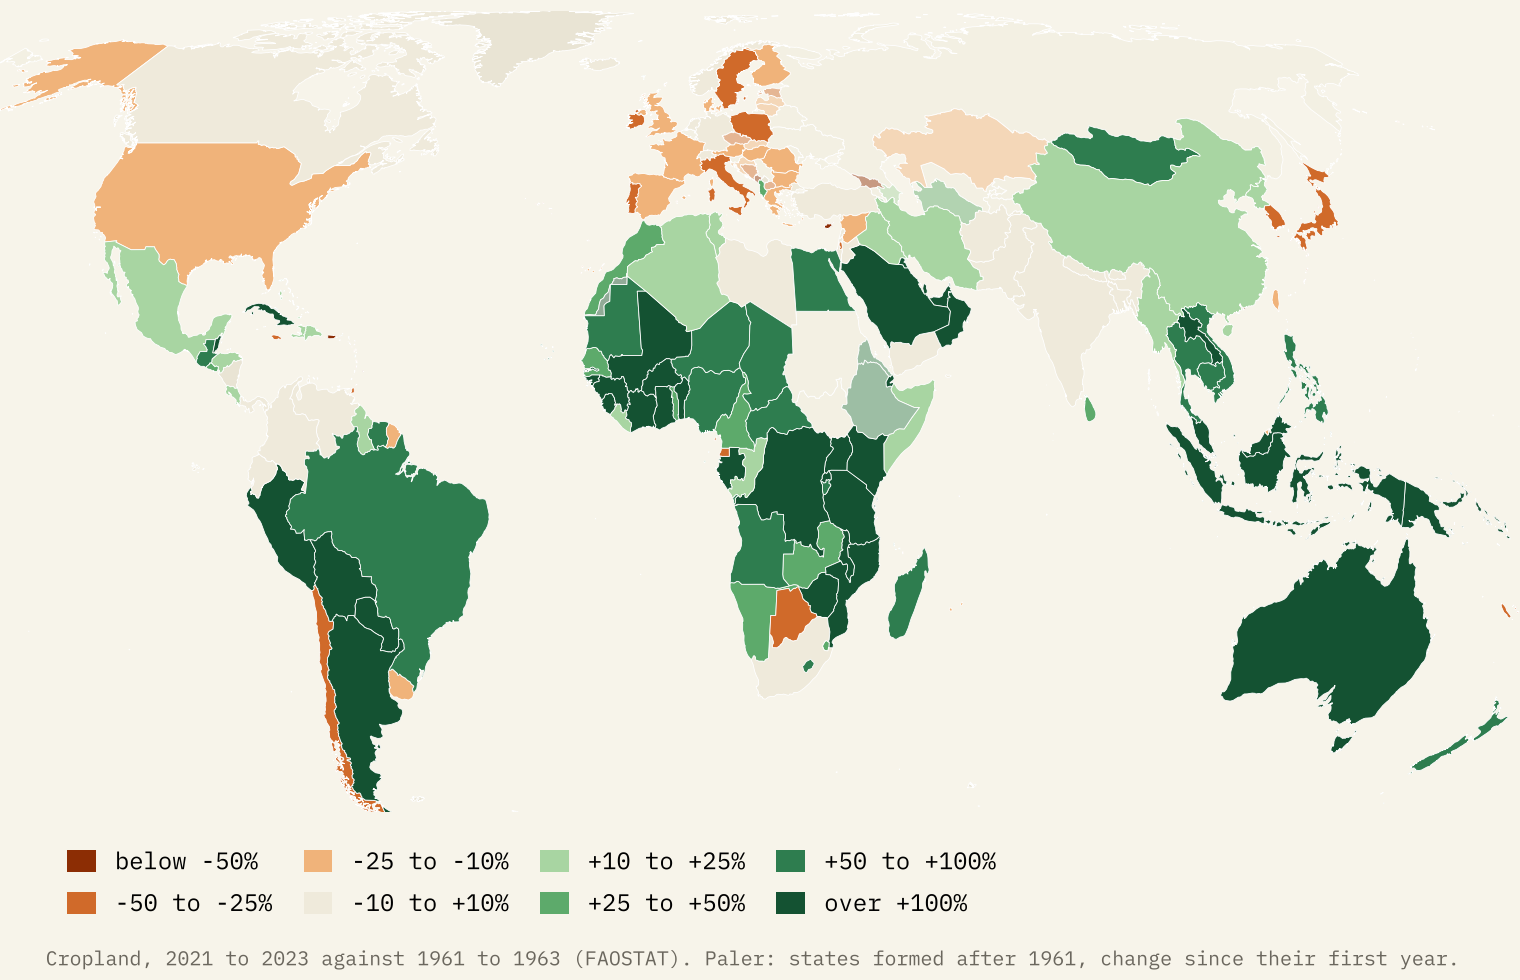
\includegraphics[width=\textwidth]{f_change_map.png}
\caption{Change in cropland, 2021 to 2023 against 1961 to 1963.}\label{fig:change}\end{figure}

\subsection{Which crops}
FAOSTAT records 1,493 million hectares harvested in 2024, 54\% more than in 1961. Wheat (220 million hectares), maize (210), rice (172) and soya beans (143) cover 50\% of it (Figure~\ref{fig:crops}). Of the extra 521 million hectares since 1961, soya beans, oil palm and maize account for 48\%. In relative terms the fastest growth among the 34 crops was in yams (×9.5, driven by Nigeria), oil palm (×8.0), rapeseed (×6.8), cowpeas and soya beans (×6.0). Rye ($-$88\%) and oats ($-$78\%) shrank most.

\begin{figure}[tbp]\centering\includegraphics[width=.84\textwidth]{f_crops_change.png}
\caption{Harvested area of the 34 crops in 2024 (bars) and 1961 (ticks), FAOSTAT.}\label{fig:crops}\end{figure}

\subsection{Where}
Figure~\ref{fig:dom} shows the dominant crop of each 0.1 degree square. Wheat leads on 26\% of farmed squares, maize on 23\%, rice on 10\% and soya beans on 8\%; cereals lead on 68\%, oilseeds on 14\% and tree crops on 9\%. The familiar belts are clear (Figure~\ref{fig:belts}): 85\% of the world's rice area is in South, Southeast and East Asia; 74\% of soya beans in the Americas, 68\% in Brazil, the United States and Argentina; 67\% of oil palm in Indonesia and Malaysia; and 66\% of cocoa in West Africa, 46\% in Côte d'Ivoire and Ghana.

\begin{figure}[tbp]\centering\includegraphics[width=\textwidth]{f_dominant_map.png}
\caption{Dominant crop by harvested area in each 0.1 degree square, CROPGRIDS around 2020. Opacity rises with the share of land harvested.}\label{fig:dom}\end{figure}

\begin{figure}[tbp]\centering\includegraphics[width=\textwidth]{f_belts.png}
\caption{Harvested area of six crops as a share of each square's land, CROPGRIDS.}\label{fig:belts}\end{figure}

Harvested area is highly concentrated (Figure~\ref{fig:conc}): half lies on 6.4\% of the world's land and nine tenths on 21\%. Within farmed squares, one crop takes at least half the harvested area in squares holding 53\% of the total. The area-weighted mean diversity is 4.0 effective crops (Figure~\ref{fig:div}); by country it is highest in Belarus (7.4), Haiti, the Central African Republic and Nigeria, and lowest in Malaysia (1.8), Afghanistan, Kazakhstan and Bangladesh. The United Kingdom scores 4.4, the United States 2.5.

\begin{figure}[tbp]\centering\includegraphics[width=.86\textwidth]{f_concentration.png}
\caption{Cumulative share of harvested area against share of land, squares ranked by harvested area per hectare.}\label{fig:conc}\end{figure}

\begin{figure}[tbp]\centering\includegraphics[width=\textwidth]{f_diversity_map.png}
\caption{Effective number of crops (of the 34) in each farmed square.}\label{fig:div}\end{figure}

\subsection{Countries: biggest crops and specialities}
Wheat is the biggest crop by area in 42 of 198 countries, maize in 32, rice in 22 and coconuts in 17, all island states (Figure~\ref{fig:top}). Soya beans lead in the United States, Brazil and Argentina; sunflower in Ukraine; oil palm in Indonesia and Malaysia; cocoa in Côte d'Ivoire; olives in Spain and Tunisia.

\begin{figure}[tbp]\centering\includegraphics[width=\textwidth]{f_top_crop_map.png}
\caption{Crop with the largest harvested area in each country, 2022 to 2024.}\label{fig:top}\end{figure}

Specialities (Figure~\ref{fig:spec}) are more distinctive. Saudi Arabia gives 34\% of its harvested area to dates, 374 times the world share. Madagascar's vanilla holds 80\% of the world's vanilla area; Bolivia's quinoa 68\%; Türkiye's hazelnuts 69\%; France's flax 53\%. Some specialities are big crops: soya beans in the United States, sunflower in Ukraine, rubber in Thailand, cocoa in Côte d'Ivoire, yams in Nigeria (73\% of the world's yam area).

\begin{figure}[tbp]\centering\includegraphics[width=.84\textwidth]{f_specialities.png}
\caption{Specialities of selected countries: the crop with the highest location quotient.}\label{fig:spec}\end{figure}

\subsection{The United Kingdom}
Pasture covers 45\% of the UK's land and cropland 25\%; cropland is 17\% smaller than in 1961 to 1963. Wheat, barley and rapeseed fill 76\% of harvested area, wheat 40\%. On the 0.05 degree grid, and leaving out maize (below), wheat leads in squares holding 57\% of UK harvested area and barley 40\% (Figure~\ref{fig:uk}). Over sixty years oats fell from 704,292 to 182,046 hectares and potatoes from 303,000 to 118,407, while rapeseed rose from 600 hectares to a peak of 755,717 in 2012 and field beans from 600 to 135,387 (Figure~\ref{fig:ukser}). Field and broad beans are the UK's speciality (24 times the world share).

\begin{figure}[tbp]\centering\includegraphics[width=\textwidth]{f_uk_crops.png}
\caption{Five UK crops at 0.05 degrees, CROPGRIDS; totals are CROPGRIDS harvested area.}\label{fig:uk}\end{figure}

\begin{figure}[tbp]\centering\includegraphics[width=.86\textwidth]{f_uk_series.png}
\caption{UK harvested area by crop, 1961 to 2024, FAOSTAT.}\label{fig:ukser}\end{figure}

\section{How detailed can we get?}
The finest open global picture is CROPGRIDS at 0.05 degrees: 2,851,739 cells hold at least one of these crops. But resolution is not the same as detail. Many inputs were coarser and were spread across finer cells, so the effective detail is often closer to 10 km, which is why the atlas uses 0.1 degree squares. The area-weighted quality score for these crops is 0.79 out of 1, lowest for sesame (0.47), rubber, oats and rye. Summed by country, CROPGRIDS agrees well with FAOSTAT 2020 (Pearson correlation 0.99 of log totals across 166 countries; CROPGRIDS totals 97\% of FAOSTAT's area for these crops), but single crops in single countries can differ widely. The clearest case is maize in north-west Europe: CROPGRIDS places 830,562 hectares of maize in the United Kingdom, 347,963 in Finland and 96,946 in Ireland, where FAOSTAT records no grain maize, all from one European source dataset; it is probably silage maize. I leave maize out of the UK analysis and flag it on the map. Over time, the detail falls to the country and the year: FAOSTAT since 1961, with breaks where states split.

\section{Limitations}
First, area is not output: a hectare of wheat in Kazakhstan counts as much as a hectare of greenhouse tomatoes. Second, the 34 crops leave out vegetables, most fruit, fodder crops and grass, which matters for diversity and for countries such as the Netherlands. Third, CROPGRIDS is a model with known errors and a single nominal year; it should not be read cell by cell. Fourth, FAOSTAT figures for many countries are estimates or imputed, and land-use definitions (especially of pasture) vary between countries. Fifth, location quotients exaggerate small crops in countries with little farmland, which is why I set minimum areas.

\section{Conclusion}
Open data now allow a credible map of what the world grows at roughly 10 km, and a country-level record of change over six decades. Together they show farmland that is mostly grass, cropland that has moved from Europe and North America into the tropics, a harvest dominated by four crops and increasingly by oil and feed, and production concentrated on a small share of the world's land. The atlas lets readers explore each of these, while the data's limits remain visible.

\section*{Data and code availability}
The interactive atlas is at \url{https://maps.tristanhotham.com/crop-map/}. Data and code are at \url{https://github.com/Tristan-Hotham/crop-map} and archived with this paper at \url{https://doi.org/{{DOI}}}. Derived data are released under CC BY 4.0 and code under the MIT licence. CROPGRIDS and FAOSTAT are both CC BY 4.0.

\section*{AI statement}
I wrote the text, with drafting and editing assistance from Claude (Anthropic), which also helped prepare the analysis code. I reviewed and checked all text and results.

\begin{thebibliography}{9}
\bibitem[FAO(2026)]{faostat} FAO (2026) FAOSTAT: Crops and livestock products; Land use. Food and Agriculture Organization of the United Nations, Rome. CC BY 4.0. \url{https://www.fao.org/faostat/}
\bibitem[Monfreda et al.(2008)]{monfreda} Monfreda, C., Ramankutty, N. and Foley, J.A. (2008) Farming the planet: 2. Geographic distribution of crop areas, yields, physiological types, and net primary production in the year 2000. \emph{Global Biogeochemical Cycles}, 22, GB1022.
\bibitem[Natural Earth(2026)]{naturalearth} Natural Earth (2026) Admin 0 countries and populated places. Public domain. \url{https://www.naturalearthdata.com/}
\bibitem[Tang et al.(2024)]{cropgrids} Tang, F.H.M., Nguyen, T.H., Conchedda, G., Casse, L., Tubiello, F.N. and Maggi, F. (2024) CROPGRIDS: a global geo-referenced dataset of 173 crops. \emph{Scientific Data}, 11, 413. \url{https://doi.org/10.1038/s41597-024-03247-7}. Data: figshare, article 22491997, CC BY 4.0.
\bibitem[Yu et al.(2020)]{spam} Yu, Q., You, L., Wood-Sichra, U. et al. (2020) A cultivated planet in 2010, part 2: the global gridded agricultural-production maps. \emph{Earth System Science Data}, 12, 3545 to 3572.
\end{thebibliography}
\end{document}
